\chapter{Simulation} 

In this section, there will be two subsections.  One will discuss the simulation to validate our design and implementation.  The other will be used to test the performance using parametric studies.  These two will be explained in the following subsequent section \ref{sec:scenario1} and \ref{sec:scenario2}.
%Various scenarios are to be tested as discussed in section \ref{sec:scenarios}.

%When simulating each scenario, the following metrics will be measured:
%\begin{enumerate}
%	\item Time to update state in central repository (delay)
%	\item Variation in time to update state (delay jitter)
%	\item Number of state updates lost. Roughly corresponds to packet loss.
%	\item Memory utilization and packet dropping threshold within ferries.
%\end{enumerate}


%________________________SCENARIO 1_______________________________
\section{Scenario 1: Validation}
\label{sec:scenario1}

In this scenario, we are trying to test to validate our design implementation, we need to address what to look for.  We need to validate that the updates from source nodes are delivered successfully when in range and to see if the packets are handled properly as designed.  

\subsection{Topology}

The topology used is to test if the message ferrying design is working properly.  There is two gateway nodes, two ferry nodes, and seven source nodes.  The paths of the ferry movement is outlined in white color.  

%picture of the rectangular path
\begin{figure}[h]
    \centering
    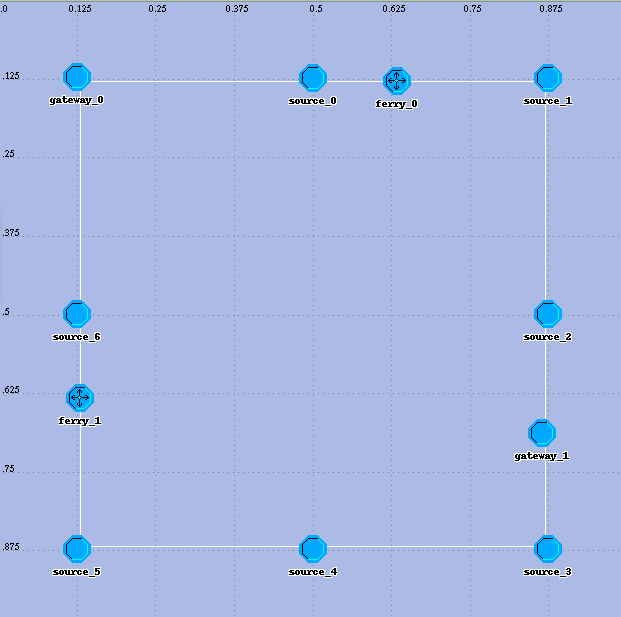
\includegraphics[width=.5\textwidth]{images/scenario1-test}
    \caption{Scenario1 Topology}
    \label{fig:scenario1}
\end{figure}
test cite ~\cite{s:wearable}

\subsection{Simulation 1 Results}

\subsection{Discussion}





%________________________SCENARIO 2_______________________________
\section{Scenario2 : Performance Evaluations}
\label{sec:scenario2}

Forthe performance evaluations, we can determine the memory utilization versus the packet dropping threshold within ferries.  

\subsection{Scenario Considerations}

The following factors have been considered when designing scenarios.
\begin{itemize}
\item Number of sources to ferries to gateways (various ratios)
\item Speed and trajectories of ferries (random vs set path)
\item Rate of source node state changes
\item Buffer size of ferries and size of property values (affects packet sizes)
\item Distances and distributions of ferries and gateways
\end{itemize}

\subsection{Scenario 2: Topology}

What is the scenario features. 
What specifically is it trying to test or measure.

List other scenarios

\section{Results}

Show result tables and graphs.
Discuss implications.
